\documentclass[11pt]{article}

%
% Everything regarding figures
\usepackage{bm, amsmath, amsthm, amssymb} %for definitions and theorems...
\usepackage{color}

\usepackage{url}
\usepackage{comment}

%\newtheorem{thm}{Theorem}[section]
%\newtheorem{cor}[thm]{Corollary}
%\newtheorem{lem}[thm]{Lemma}

%\theoremstyle{remark}
%\newtheorem{rem}[thm]{Remark}

\theoremstyle{definition}
\newtheorem{def2}[]{Definition}

\usepackage{graphicx}
\usepackage{amssymb}


\usepackage{hyperref}

\hypersetup{
  colorlinks,
  citecolor=violet,
  linkcolor=red,
  urlcolor=blue}

% nikos \setcounter{topnumber}{3}
% nikos \setcounter{bottomnumber}{3}
% nikos \setcounter{totalnumber}{3}

 
%
% If you like postscript fonts more than computer modern

% \usepackage{newcent}

 
% ==========   Local defs and mods
%

% nikos \usepackage{alltt}
% nikos \setcounter{tocdepth}{1}  % chapter, sections to toc
% nikos\newenvironment{demo}
% nikos  {\begin{alltt}\leftskip3em
% nikos     \def\\{\ttfamily\char`\\}%
% nikos     \def\{{\ttfamily\char`\{}%
% nikos     \def\}{\ttfamily\char`\}}}
% nikos  {\end{alltt}}

% metafont font.  If logo not available, use the second form
%
% \font\mffont=logosl10 scaled\magstep1
\let\mffont=\sf
\DeclareGraphicsExtensions{.png,.PNG,.jpg,.JPG,.pdf,.PDF}
% registered symbol.
%
\def\registered{\setlength{\unitlength}{1cm}
\begin{picture}(0.3,0.3) 
        \put(0.0,0.4) {\circle{0.4}\makebox(-0.3,0.1)[tr]{\tiny R}}
\end{picture}}

\usepackage{graphicx}
\usepackage{color}
\usepackage{wrapfig}
\usepackage{amssymb}
\usepackage{amsmath}
\usepackage{amsfonts}
\usepackage{subfigure}
\usepackage{float}
\usepackage{wrapfig}


\textwidth      6.70in
\oddsidemargin  -0.0in
\evensidemargin -0.0in

\textheight     9.20in
\headheight     0in
\headsep        0in
\topmargin      -0.15in

\raggedbottom


\pagestyle{empty}


\def\elept{\def\baselinestretch{0.88}\let\normalsize\large\normalsize}
\def\tenpt{\def\baselinestretch{0.88}\let\normalsize\normalsize\normalsize}
\def\ninept{\def\baselinestretch{0.88}\let\normalsize\small\normalsize}
\def\eightpt{\def\baselinestretch{0.88}\let\normalsize\footnotesize\normalsize}
\def\sevenpt{\def\baselinestretch{0.88}\let\normalsivvze\scriptsize\normalsize}
\def\sixpt{\def\baselinestretch{0.88}\let\normalsize\tiny\normalsize}

\newcommand{\bumpup}{\vspace*{-1.2ex}}

\begin{document}

\tenpt

\newcommand{\pxmark}{{\normalsize *}}
 \newcommand{\px}{\makebox[0pt][r]{\pxmark{\hspace*{.5pt}}}}

\pagestyle{plain}



%\psdraft
\setlength{\itemsep}{-\parsep}\setlength{\topsep}{-\parsep}
\tenpt
\section{Executive Summary}\label{Overview}
\vspace{-0.15in} 

are seeking \$50,000 in seed funding for our Minnesota based asdf company, RedLeaf. This funding will accelerate the development of our first product, a "smart" cooking device for consumers. Cooking is a fundamental human activity that is performed daily by most of the population, yet cooking devices have not kept pace with the rapid advances in digital technology. The device improves the cooking experience through more control, more information provided to the user and the ability to precisely share cooking methods from user to user. These capabilities are made possible by applying the latest  embedded computers, control algorithms and sensors. 

\section{Technology Description}

%Hardware
%Software
%Application





\section{Markets}

The market potential for a cooking device is 

 A study by the Organization of Economic Cooperation and Development  (OECD) in 2011 found that 55\% of the US population (182 million) cooks on an average day \cite{cooktime}. This study also found that the average American spends 1 hour 44 minutes preparing and eating food. An average of 30 minutes a day on food preparation alone. A study by the USDA with data from 2006-2008 confirms these results, which found 54\% of Americans cook on an average day and spend 33 minutes on food preparation \cite{usdacooktime}. A study by the Department of Nutrition at the University of North Carolina Gillings School of Global Public Health reported from 1965 to 1990 the amount of time spent on cooking preparation declined due to eating out and cooking technologies, but has since plateud at a the again confirmed, over half of US adults cooking on a given day. A Harris Marketing research pole found 89\% of US adults prepare meals at home more 1-2 times or more per week and 60\% more than 3-4 times per week \cite{harris_food_stats}. This study also found three in ten US adults reported that they "love to cook."  

The market can be analyzed in terms of customer segments. Each of these are outlined as follows:

\begin{enumerate}
\item Consumer shopping for cooking appliances
\begin{enumerate}
	\item Consumer shopping for large cooking appliance
	\item Consumer shopping for small surface cooking units
\end{enumerate}
\item Consumers not shopping for a cooking appliance
	\begin{enumerate}
		\item Technology connoisseurs
		\item Cooking connoisseurs
		\item Special Interest Food Preparation
		\item Customers That Desire Simpler, Quicker Food Preparation
		\item Other
	\end{enumerate}
\end{enumerate}


Consumers shopping for large cooking appliances are typically renovating their home or making a new home purchase. The total volume sold in this market for cooking appliances including electric and gas ranges, surface units and ovens as well as microwaves was 16,521,000 in 2012 according to Appliance Magazine \cite{appmag}. The total surface units sold including ranges was 6,315,000. This provides an idea of the annual turnover of cooking appliances and surface units.

The market size of consumers shopping for small surface cooking units is typically viewed as an accessory item for a specific use or in replacement of a large appliance. 
Bloomberg reported that, based on NPD Group Inc. research, small kitchen-appliance experienced a surge of 10\% in purchases in 2012 to a market size of \$5.51billion. This growth beat last years increase of 9.4\% with 132.2 million units sold. A significant portion of these sales were high-end speciality appliances with gross margins above 30\%.

These statics support the RedLeaf Hypothesis well. To the best of our knowledge, the RedLeaf cooktop will be the most accurate, high tech cooking appliance on the market. 


Based on a study by PackagedFacts on Market Research Bureau data, 31 Million adults in the US (14\% of the population) fall into a consumer category that has been called "foodies" or food aficionados \cite{foodie_facts}. These are people who consider food and cooking a hobby rather than a necessity. These consumers enjoy high-end gourmet food and embrace food-related trends..  On Pinterest (20 million unique visitors per day), 57\% of posts  are food related, 70\% of account holders cite cooking and recipes as the top item they pin. 


\subsection{Competitors}








\subsection{Emerging Demand for Internet of Things}

The internet of things (IoT) has been dubbed a "quiet revolution" and is a sweeping. The internet of things refers the ability to connect physical systems to the internet and provide and receive information from users or other systems. According to a study by The Economist \cite{iot}, 76\% of surveyed companies are exploring IoT for internal uses (operations and processes), and 74\% for external products or services. For consumer products one of the best examples of how IoT is being applied is the Nest Thermostat (\href{https://nest.com/}{nest.com})  shown in Figure~\ref{fig:nest}. The Nest Thermostat retails for \$249 and provides an automated learning function and allows for the control home heating from a smartphone or computer with an internet connection. Nest was shipping 40,000 units per month in January, 2013 \cite{nest_sales} and is reportedly, pursuing a financing round with a valuation of over \$2B\cite{nest_valuation}.

%Nest thermostat




%Reasons someone would purchase

\begin{wrapfigure}{r}{0.5\textwidth}
   \begin{center}
     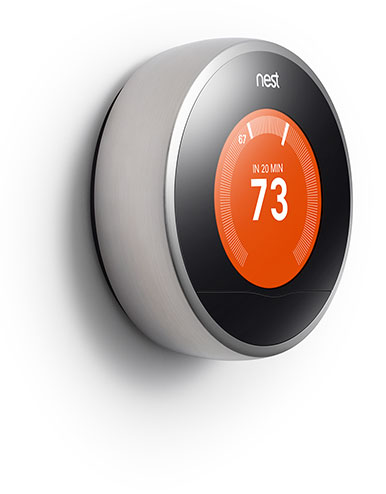
\includegraphics [height=0.5\textwidth,width=3in]{nest.jpg}
   \end{center}
\vspace{+0.2in}
   \caption{Nest Thermostat
   \label{fig:nest}}
\vspace{-10pt}
\end{wrapfigure}


%Nomiku/suis vide




\subsection{Competition}

%Accessory Appliances

%Major Appliance Manufacturers



\subsection{Distribution}

\begin{wrapfigure}{r}{0.5\textwidth}
   \begin{center}
     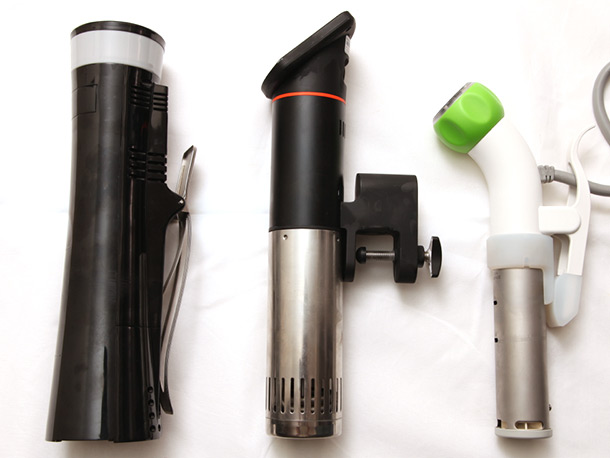
\includegraphics [height=0.3\textwidth,width=3in]{suis_vide.jpg}
   \end{center}
\vspace{+0.2in}
   \caption{Sous vide cookers \label{fig:nomiku}}
\vspace{-10pt}
\end{wrapfigure}



	Several recent product launches in specialty items provide a good example of consumer demand for specialty high tech cooking devices. A sous vide cooker maintains the water temperature to slowly cook food to produce a distinct texture and taste. Nomiku successfully launched their product through a \href{http://www.kickstarter.com/projects/seattlefoodgeek/sansaire-sous-vide-circulator-for-199}{ kickstarted campaign} that raised \$586,000 with a majority of the funds raised through pre orders of their product at \$299 per unit (shown furthest right in figure~\ref{fig:nomiku}) . Within 6 months another 2 sous vide cookers were launched on a \href{http://www.kickstarter.com/projects/seattlefoodgeek/sansaire-sous-vide-circulator-for-199}{kickstarter} which raised \$823,000 (shown furthest left in Figure~\ref{fig:nomiku}). These successful campaigns show two relevant pieces of information for the RedLeaf concept. The first is the demand for specialty cooking devices. A sous vide cooker is highly specialized and can cook very limited types of foods. The second is that combined this concept raise over \$1.2 million during their kickstarter campaigns, which requires customers to pay upfront and wait up to a year to receive the product. Further both of these startup companies (nomiku.com and sansaire.com) continued to accept pre orders through direct sales via their website. 

%Direct Sales
%Retail
%Amazon




\section{Company Summary}

RedLeaf plans to apply recent advances robotics, low cost embedded systems and uncompromising aesthetic design to add value to consumer products already in the market, and to develop new product concepts that are found feasible through this model.


\subsection{Business Model}

Since RedLeaf is selling physical products the business model is quite simple. The only difference between revenues and costs purely associated with manufacturing and sales is the development of an web based application. For products where shared knowledge and crowd based voting may add value to the product, we plan to include web applications to make this possible. The reason for offering it at no cost is that we believe this will be a major driver to new customer aquisition.

The first product being developed is the most advanced yet simplest cooking device in the consumer market.

In a nutshell it is a burner which intelligently senses and controls the temperature of cooking surface. What this means for the user is that they are able to cook food both with greater accuracy, repeatability and simplicity.





The implementation strategy will be through rapidly prototyping concepts, pre-order launches, validation stages and progressive manufacturing runs. The goal is to maximize the ideas considered, minimize bureaucratic effects, use hard data to make decisions and minimize risk associated with design for manufacturing, fabrication tooling and distribution. This strategy can be visualized in figure 1.

The ongoing rapid advancement of �smart phone� technologies has driven down embedded computer costs and form factors. RedLeaf was formed on the basis that there is a discrepancy between current consumer devices and appliances, and the value that could be added through low cost embedded systems. 

RedLeaf�s team has a strong background in robotics research, which has provided deep insight into the problems that robotics algorithms and intelligence are able to make great value propositions and which are not yet practical.

The final component of RedLeaf is prioritizing aesthetic design. We will let our founding members ability to accomplish great aesthetic design speak for itself in terms of our first product, but long term we deem this essential to the success of the company brand and a major differentiator with potential competition. RedLeaf will be a premium brand, which requires that the product to look as appealing as it is functional. Long term this will include a heavy emphasis and recruiting and curating the talented product designers.

RedLeaf was founded in the summer of 2013 by Ruben D�Sa and Scott morton. Since then the company has been developing its first product that is targeting the small appliance and accessory appliance markets. During November of 2013 a third team member joined, Sandeep D�Hull, in order to add advanced embedded system development capabilities to the team.



\section{The Founders}




\section{Timeline}





\section{Financial Plan}







\section{Appendix}

\begin{thebibliography}{}


\bibitem{smappliances}
\url{http://www.euromonitor.com/small-cooking-appliances-in-the-us/report}


\bibitem{appmag}
\url{http://www.appliancemagazine.com/marketresearch/editorial.php?article=2431&zone=108&first=21}



\bibitem{cooktime}
 \url{http://www.oecd.org/social/soc/47571423.pdf}

\bibitem{euromonitor}
\url{http://www.euromonitor.com/small-cooking-appliances-in-the-us/report}

\bibitem{bloomberg}
\url{http://www.bloomberg.com/news/2013-04-05/macy-s-600-blenders-win-boomers-in-kitchen-gadget-surge.html}

\bibitem{iot}
\url{http://www.arm.com/files/pdf/EIU_Internet_Business_Index_WEB.PDF}

\bibitem{pinterestfood}
\url{http://therealtimereport.com/2012/04/02/pin-commerce-21-of-pinterest-users-have-purchased-a-product-they-found-on-the-site/}

\bibitem{nest_com}
\url{https://nest.com/thermostat/life-with-nest-thermostat/}

\bibitem{nest_sales}
\url{http://gigaom.com/2013/01/29/exclusive-nest-has-raised-another-80m-now-shipping-40k-thermostats-a-month/}

\bibitem{nest_valuation}
\url{http://recode.net/2014/01/02/nest-raising-huge-new-round-from-dst-valuing-smart-home-startup-at-upwards-of-2-billion/}

\bibitem{foodie_facts}
\url{http://www.packagedfacts.com/Foodies-Cohorts-Foreign-1653977/}

\bibitem{usda_cooktime}
\url{http://www.ers.usda.gov/publications/eib-economic-information-bulletin/eib86.aspx#.UshRVWRDuUc}

\bibitem{food_stats}
\url{http://www.ncbi.nlm.nih.gov/pmc/articles/PMC3639863/}

\bibitem{harris_food_stats}
\url{http://www.harrisinteractive.com/NewsRoom/HarrisPolls/tabid/447/mid/1508/articleId/444/ctl/ReadCustom%20Default/Default.aspx}


\end{thebibliography}

\end{document} 

	